% =====================================================================
% create.project: One-Call Reproducible Research Projects, R Packages and Papers
% generated by create_paper() on 2026-10-23: edit freely, it is yours now
% compile: latexmk -pdf main.tex   (or tinytex::latexmk("main.tex", bib_engine = "biber"))
% =====================================================================
\documentclass[12pt,a4paper]{article}

% ---- Encoding, language, fonts --------------------------------------
\usepackage[T1]{fontenc}        % proper hyphenation of accented words
\usepackage[utf8]{inputenc}     % default since 2018, kept for old installs
\usepackage[english]{babel}     % hyphenation rules; also needed by biblatex-apa
\usepackage{lmodern}            % vector version of the default font
\usepackage{microtype}          % better spacing and line breaks, for free

% ---- Layout ---------------------------------------------------------
\usepackage[top=3cm, bottom=3cm, left=3cm, right=3cm]{geometry}
\usepackage{setspace}
\onehalfspacing

% ---- Maths ----------------------------------------------------------
\usepackage{amsmath,amssymb,amsfonts}

% ---- Figures --------------------------------------------------------
\usepackage{graphicx}           % \includegraphics
\usepackage{subcaption}         % subfigures with their own (a), (b) captions
\usepackage{caption}
\captionsetup{font=small, labelfont=bf}
\usepackage{float}              % [H] placement when you really need it
\usepackage{pdflscape}          % \begin{landscape} for wide tables
\usepackage{tikz}
\usetikzlibrary{positioning, arrows.meta}
\graphicspath{{figures/}}   % figures are produced by the R scripts: point to them, do not copy

% \safegraphic[options]{file}: includes the figure if it exists, otherwise
% draws a box with the missing file name, so the paper always compiles
\newcommand{\safegraphic}[2][width=\linewidth]{%
  \IfFileExists{figures/#2}%
    {\includegraphics[#1]{#2}}%
    {\fbox{\parbox[c][4cm][c]{0.9\linewidth}{\centering\small\ttfamily missing: \detokenize{#2}}}}%
}

% ---- Tables ---------------------------------------------------------
\usepackage{booktabs}           % \toprule \midrule \bottomrule: no vertical lines
\usepackage{threeparttable}     % notes under a table, aligned with it
\usepackage{multirow}

% ---- Colours, lists, quotes -----------------------------------------
\usepackage{xcolor}
\usepackage{enumitem}
\usepackage{csquotes}           % \enquote{...}, required by biblatex

% ---- Code -----------------------------------------------------------
\usepackage{listings}           % \begin{lstlisting} ... \end{lstlisting}, \lstinline|code|
\lstset{
  language         = R,
  alsoletter       = {._},      % R names contain . and _ (install_github, my.pkg)
  basicstyle       = \ttfamily\small,
  keywordstyle     = \color{blue!60!black},
  commentstyle     = \color{gray},
  stringstyle      = \color{green!40!black},
  frame            = single,
  framesep         = 4pt,
  breaklines       = true,
  columns          = fullflexible,
  keepspaces       = true,
  showstringspaces = false
}

% ---- Bibliography ---------------------------------------------------
\usepackage[backend=biber, style=apa, natbib=true]{biblatex}
\addbibresource{references.bib}

% ---- Links: hyperref last, cleveref right after ---------------------
\usepackage{hyperref}
\hypersetup{
  colorlinks = true,
  linkcolor  = blue!50!black,
  citecolor  = blue!50!black,
  urlcolor   = red!60!black,
  pdftitle   = {create.project: One-Call Reproducible Research Projects, R Packages and Papers},
  pdfauthor  = {Simon Labarthe}
}
\usepackage[capitalise, noabbrev]{cleveref}  % \cref{fig:dag} -> "Figure 1"

% ---- Writing helpers ------------------------------------------------
\newcommand{\todo}[1]{\textcolor{red}{[TODO: #1]}}   % delete before submitting

%=====================================================================%

\title{\textbf{create.project: One-Call Reproducible Research Projects, R Packages and Papers}\thanks{Word count: about 1,000.}}
\author{Simon Labarthe}
\date{October 2026}

\begin{document}

\maketitle

\begin{abstract}
Setting up an R project properly takes time: folders, git, pinned package versions, a license, a paper. Most people skip it and pay for it later. \texttt{create.project} does it in one call. \texttt{create\_project()} builds either a research project (a numbered data pipeline with \texttt{renv}) or an R package (the standard layout, with tests), and makes the first git commit. \texttt{create\_paper()} writes a LaTeX paper skeleton, for research or for software, that compiles on day one. Every step skips what already exists, so re-running is safe. The package is about 300 lines of R on top of \texttt{usethis}, \texttt{renv} and \texttt{gert}, and is open source under the MIT license.

\medskip
\noindent\textbf{Keywords:} R, reproducibility, project templates, research workflow, LaTeX
\end{abstract}

\newpage

% =====================================================================
\section{Statement of Need}\label{sec:need}

Good practices for research code are well known: keep raw data read-only, number the scripts in execution order, pin package versions, use version control, and generate figures instead of pasting them \citep{wilson2017, marwick2018}. They are also slow to set up, and the setup happens at the worst moment: the start of a project, when nothing seems at stake yet. So each project gets a different layout, or none.

\texttt{create.project} makes the good default the fast default. It targets social scientists who write R, and anyone who writes small R packages. One call gives a project that a colleague, a reviewer, or the same person on another computer can rerun.

% =====================================================================
\section{State of the Field}\label{sec:field}

\texttt{usethis} \citep{usethis} provides the building blocks (create a package, add a license, add tests) but no research layout and no paper. \texttt{rrtools} \citep{marwick2018} turns a research project into a package (a \enquote{research compendium}) with an R Markdown paper and Docker. \texttt{ProjectTemplate} \citep{projecttemplate} gives a data analysis layout. \texttt{workflowr} \citep{blischak2019} turns R Markdown analyses into a versioned website (\cref{tab:comparison}).

\texttt{create.project} sits between them: research and package layouts behind one function, and a LaTeX paper rather than R Markdown. Users who write in R Markdown or Quarto are better served by \texttt{rrtools} or \texttt{workflowr}.

\begin{table}[htbp]
    \centering
    \small
    \caption{Comparison with existing tools}
    \label{tab:comparison}
    \begin{tabular}{lccccc}
        \toprule
                         & \texttt{create.project} & \texttt{usethis} & \texttt{rrtools} & \texttt{ProjectTemplate} & \texttt{workflowr} \\
        \midrule
        Research layout  & \checkmark &            & \checkmark & \checkmark & \checkmark \\
        Package layout   & \checkmark & \checkmark & \checkmark &            &            \\
        Paper            & LaTeX      &            & R Markdown &            & R Markdown \\
        Version pinning  & \texttt{renv} &         & Docker     &            &            \\
        \bottomrule
    \end{tabular}
\end{table}

% =====================================================================
\section{Design}\label{sec:design}

\subsection{Principles}

\begin{enumerate}[nosep]
    \item \textbf{One call, sensible defaults.} Author, license and branch name are preset. The only required argument is the folder.
    \item \textbf{Idempotent.} Every step skips what already exists. Re-running never overwrites work, and an existing folder can be upgraded.
    \item \textbf{Delegate.} Files are created by \texttt{usethis}, environments by \texttt{renv} \citep{renv}, commits by \texttt{gert} \citep{gert}. The package only decides \emph{what} to create.
    \item \textbf{The paper compiles on day one.} Placeholders in brackets are writing guidance; example figures and tables (Star Wars data) fill the blanks; a missing figure is drawn as a labelled box instead of breaking the build.
\end{enumerate}

\subsection{Architecture}

Two exported functions (\cref{fig:architecture}). \texttt{create\_project()} chooses a layout from \texttt{type}, then calls \texttt{create\_paper()} with the matching paper type. \texttt{create\_paper()} also works alone, in any project. \Cref{tab:layouts} lists what each layout contains.

\begin{figure}[htbp]
    \centering
    \footnotesize
    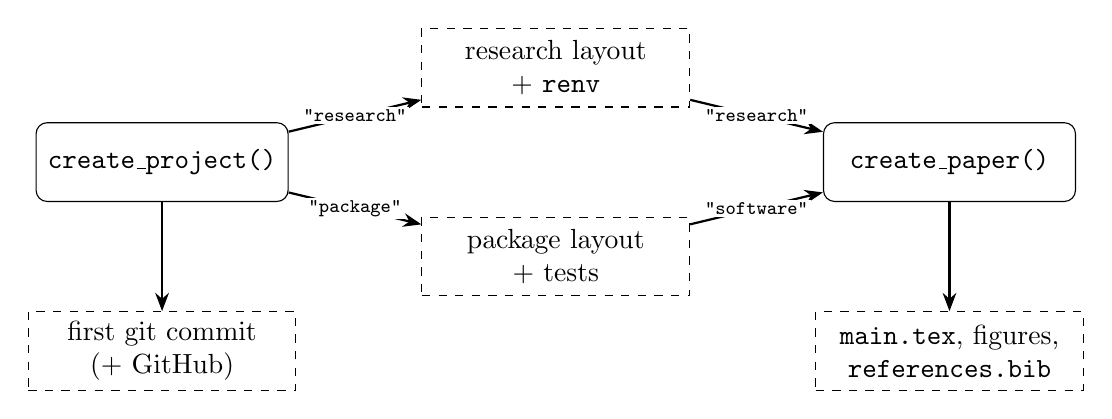
\begin{tikzpicture}[box/.style={draw, rounded corners, align=center, minimum width=3.2cm, minimum height=1cm},
                        result/.style={draw, dashed, align=center, minimum width=3.4cm, minimum height=1cm}]
        \node[box]    (cp)  at (0,0)     {\texttt{create\_project()}};
        \node[result] (res) at (5,1.2)   {research layout\\+ \texttt{renv}};
        \node[result] (pkg) at (5,-1.2)  {package layout\\+ tests};
        \node[box]    (pp)  at (10,0)    {\texttt{create\_paper()}};
        \node[result] (tex) at (10,-2.4) {\texttt{main.tex}, figures,\\\texttt{references.bib}};
        \node[result] (git) at (0,-2.4)  {first git commit\\(+ GitHub)};

        \tikzset{lab/.style={midway, fill=white, inner sep=1pt, font=\scriptsize\ttfamily}}
        \draw[-{Stealth}, thick] (cp)  -- node[lab] {"research"} (res);
        \draw[-{Stealth}, thick] (cp)  -- node[lab] {"package"}  (pkg);
        \draw[-{Stealth}, thick] (res) -- node[lab] {"research"} (pp);
        \draw[-{Stealth}, thick] (pkg) -- node[lab] {"software"} (pp);
        \draw[-{Stealth}, thick] (pp) -- (tex);
        \draw[-{Stealth}, thick] (cp) -- (git);
    \end{tikzpicture}
    \caption{Architecture: two exported functions and what they produce}
    \label{fig:architecture}
\end{figure}

\begin{table}[htbp]
    \centering
    \small
    \caption{The two layouts}
    \label{tab:layouts}
    \begin{tabular}{ll}
        \toprule
        \texttt{type = "research"}                    & \texttt{type = "package"}                        \\
        \midrule
        \texttt{1\_raw\_data/} never edited by hand   & \texttt{R/} all functions                         \\
        \texttt{2\_scripts/} numbered = run order     & \texttt{man/} generated documentation             \\
        \texttt{3\_derived\_data/} regenerated        & \texttt{tests/testthat/} unit tests               \\
        \texttt{4\_outputs/} figures, tables          & \texttt{vignettes/} tutorial                      \\
        \texttt{5\_docs/} research paper              & \texttt{data-raw/} scripts that build \texttt{data/} \\
        \texttt{6\_archives/} old material            & \texttt{inst/CITATION}                            \\
        \texttt{renv/} pinned package versions        & \texttt{paper/} software paper                    \\
        \midrule
        \multicolumn{2}{l}{both: \texttt{DESCRIPTION}, \texttt{.Rproj}, \texttt{LICENSE}, \texttt{README.md}, ignore files, git} \\
        \bottomrule
    \end{tabular}
\end{table}

\subsection{Decisions and Trade-offs}

\begin{itemize}[nosep]
    \item \textbf{One function with \texttt{type}, not two functions.} About 80\% of the steps are shared; two functions would drift apart.
    \item \textbf{\texttt{renv} for research only.} A package declares its dependencies in \texttt{DESCRIPTION}; pinning them would fight its users.
    \item \textbf{No options that nobody used.} Flags for git, \texttt{renv} and data splits, a generated folder map and a per-computer setup function were removed: each cost code and explanation for little benefit.
    \item \textbf{The repository is named after the package} (\texttt{my.project}, not \texttt{my\_project}), because \texttt{usethis} does so and offers no override.
    \item \textbf{Example figures are drawn, not copied.} The duel in \cref{fig:output} is made with \texttt{ggplot2}; film stills are copyrighted.
\end{itemize}

% =====================================================================
\section{Usage}\label{sec:usage}

Install once, and keep \texttt{renv} libraries out of synced folders (OneDrive, Dropbox) with one line in the user \texttt{.Renviron}:

\begin{lstlisting}
remotes::install_github("SimonLabarthe/create.project")
usethis::edit_r_environ()   # add: RENV_PATHS_LIBRARY_ROOT=<local folder>
\end{lstlisting}

Then one call per project:

\begin{lstlisting}
library(create.project)

create_project("~/seminar/inequality", title = "Inequality and Repression")
create_project("~/dev/coolfun", type = "package")
create_paper("5_docs")          # only the paper, in an existing project
\end{lstlisting}

The research call writes the six folders, five numbered script templates, a paper and a first commit. The paper already contains a causal diagram, two tables and five figures (\cref{fig:output}); each is an example to replace.

\begin{figure}[htbp]
    \centering
    \begin{subfigure}{0.32\textwidth}
        \fbox{\safegraphic[width=0.95\linewidth]{demo_page3.png}}
        \caption{Causal diagram}
    \end{subfigure}\hfill
    \begin{subfigure}{0.32\textwidth}
        \fbox{\safegraphic[width=0.95\linewidth]{demo_page6.png}}
        \caption{Results}
    \end{subfigure}\hfill
    \begin{subfigure}{0.32\textwidth}
        \fbox{\safegraphic[width=0.95\linewidth]{demo_page7.png}}
        \caption{Figure grid}
    \end{subfigure}
    \caption{Three pages of a freshly generated research paper, before any writing}
    \label{fig:output}
\end{figure}

% =====================================================================
\section{Quality and Validation}\label{sec:quality}

22 \texttt{testthat} expectations cover both layouts, re-running on an existing project, the paper templates and the escaping of LaTeX special characters. \texttt{R CMD check} reports no errors, warnings or notes, and so does a package freshly generated with \texttt{type = "package"}. Both paper types compile without LaTeX warnings with \texttt{pdflatex} and \texttt{biber}. Everything was tested on Windows 11 with R 4.5.2.

% =====================================================================
\section{Limitations and Future Work}\label{sec:limits}

Defaults (author, GitHub account) are the author's own: other users must pass them as arguments. macOS and Linux are untested. Papers are LaTeX only. Next steps: read personal defaults from \texttt{options()}, add a continuous integration workflow, and offer a Quarto paper.

% =====================================================================
\section{Conclusion}\label{sec:conclusion}

Good project structure is cheap once it is one function call away. \texttt{create.project} makes that call, and gives the paper a head start.

% =====================================================================
\section*{Software Availability}
\begin{itemize}[nosep]
    \item Repository: \url{https://github.com/SimonLabarthe/create.project}
    \item Version described: 0.3.0
    \item License: MIT
    \item Requirements: R, and a LaTeX distribution (e.g.\ TinyTeX) for the papers
\end{itemize}

\newpage
\printbibliography

\end{document}
